%2multibyte Version: 5.50.0.2953 CodePage: 1252

\documentclass{article}
%%%%%%%%%%%%%%%%%%%%%%%%%%%%%%%%%%%%%%%%%%%%%%%%%%%%%%%%%%%%%%%%%%%%%%%%%%%%%%%%%%%%%%%%%%%%%%%%%%%%%%%%%%%%%%%%%%%%%%%%%%%%%%%%%%%%%%%%%%%%%%%%%%%%%%%%%%%%%%%%%%%%%%%%%%%%%%%%%%%%%%%%%%%%%%%%%%%%%%%%%%%%%%%%%%%%%%%%%%%%%%%%%%%%%%%%%%%%%%%%%%%%%%%%%%%%
\usepackage{amsfonts}
\usepackage{amsmath}
\usepackage{hyperref}
\hypersetup{
    colorlinks=true,
    linkcolor=blue,
    filecolor=magenta,      
    urlcolor=cyan,
    pdftitle={Overleaf Example},
    pdfpagemode=FullScreen,
    }

\setcounter{MaxMatrixCols}{10}
%TCIDATA{OutputFilter=LATEX.DLL}
%TCIDATA{Version=5.50.0.2953}
%TCIDATA{Codepage=1252}
%TCIDATA{<META NAME="SaveForMode" CONTENT="1">}
%TCIDATA{BibliographyScheme=Manual}
%TCIDATA{Created=Tuesday, September 13, 2016 11:26:35}
%TCIDATA{LastRevised=Tuesday, October 15, 2019 14:55:43}
%TCIDATA{<META NAME="GraphicsSave" CONTENT="32">}
%TCIDATA{<META NAME="DocumentShell" CONTENT="Standard LaTeX\Blank - Standard LaTeX Article">}
%TCIDATA{CSTFile=40 LaTeX article.cst}
\usepackage{enumitem}
\usepackage{floatrow}
\usepackage{graphicx} 
\usepackage{caption}

\newtheorem{theorem}{Theorem}
\newtheorem{acknowledgement}[theorem]{Acknowledgement}
\newtheorem{algorithm}[theorem]{Algorithm}
\newtheorem{axiom}[theorem]{Axiom}
\newtheorem{case}[theorem]{Case}
\newtheorem{claim}[theorem]{Claim}
\newtheorem{conclusion}[theorem]{Conclusion}
\newtheorem{condition}[theorem]{Condition}
\newtheorem{conjecture}[theorem]{Conjecture}
\newtheorem{corollary}[theorem]{Corollary}
\newtheorem{criterion}[theorem]{Criterion}
\newtheorem{definition}[theorem]{Definition}
\newtheorem{example}[theorem]{Example}
\newtheorem{exercise}[theorem]{Exercise}
\newtheorem{lemma}[theorem]{Lemma}
\newtheorem{notation}[theorem]{Notation}
\newtheorem{problem}[theorem]{Problem}
\newtheorem{proposition}[theorem]{Proposition}
\newtheorem{remark}[theorem]{Remark}
\newtheorem{solution}[theorem]{Solution}
\newtheorem{summary}[theorem]{Summary}
\newenvironment{proof}[1][Proof]{\noindent\textbf{#1.} }{\ \rule{0.5em}{0.5em}}
%\input{tcilatex}
\begin{document}



\begin{center}
{\Large Problem Set 6}
\end{center}


\begin{exercise} %EX12.5 SW
Consider the IV regression model
\begin{equation*}
    Y_i = \beta_0 + \beta_1 X_i + u_i
\end{equation*}
where $X_i$ is correlated with $u_i$ and $Z_i$ is an instrument. Which IV assumption is not satisfied when
\begin{enumerate}[label=\alph*)]
    \item $Z_i$ is independent of ($Y_i, X_i, W_i$)?
    \item $Z_i=W_i$
    \item $W_i = 1 \forall i$
    \item $Z_i = X_i$
\end{enumerate}
\end{exercise}


\begin{exercise} %12.7
A classmate has developed an IV regression model with one regressor, $X_i$, and two instruments, $Z_{1i}$ and $Z_{2i}$. She has a strong theoretical basis as to why $corr(Z_{1i}, u_{i2} = 0$, namely that $Z_{1i}$ is the result of a random lottery. Preliminary work, however, showed that the first-stage F-statistic from this exactly identified model was insufficiently large for $Z_{1i}$ to be considered a relevant instrument set by itself. As a result she includes an additional instrument, $Z_{2i}$, which is strongly relevant but is less likely to satisfy the condition of instrument exogeneity. In the instrumental variable regression model with one regressor, $X_i$, and two instruments, $Z_{1i}$ and $Z_{2i}$, the value of the J-statistic is $J = 7.5$.
\begin{enumerate}[label=\alph*)]
    \item Does this suggest that $\mathbb{E}(u_i \mid Z_{1i}, Z_{2i})\neq 0$? Explain.
    \item Does this suggest that $\mathbb{E}(u_i \mid Z_{2i})\neq 0$? Explain.
\end{enumerate}
\end{exercise}


\begin{exercise} %12.9
A researcher is interested in the effect of more secure property rights on income across countries. He collects recent data from 60 countries and runs the OLS regression $Y_i = \beta_0 + \beta_1 X_i + u_i$, where $Y_i$ is a country’s GDP per capita and $X_i$ is an index taking values between 0 and 10 reflecting the protection
against expropriation where a higher value indicates greater protection against expropriation, that is, more secure property rights.
\begin{enumerate}[label=\alph*)]
    \item Explain why the OLS estimates are likely to be unreliable and indicate in which direction they might be biased.
    \item All of the countries in the researcher’s sample were former colonies. Institutions securing property rights could originate from early institutions established alongside European settlements. The decision for Europeans to settle or otherwise could reflect concerns for mortality among settlers. Explain how settler mortality might be used as an instrument to estimate the effect of more secure property rights on income across countries.
\end{enumerate}
\end{exercise}


\begin{exercise} %10.2 10.3
A researcher is using a panel data set on n = 1000 workers over T = 10 years (from 2008 through 2017) that contains the workers’ earnings, sex, education, and age. The researcher is interested in the effect of education on earnings.
\begin{enumerate}[label=\alph*)]
    \item Give some examples of unobserved person-specific variables that are correlated with both education and earnings.
    \item Can you think of examples of time-specific variables that might be correlated with education and earnings?
    \item How would you control for these person-specific and time-specific effects in a panel data regression?
    \item Can the regression that you suggested in the previous answer be used to estimate the effect of a worker’s sex on his or her earnings?
    \item    Can that regression be used to estimate the effect of the national unemployment rate on an individual’s earnings? Explain.
\end{enumerate}
\end{exercise}


\begin{exercise} % 10.2
Consider the results presented in Table 1.
\begin{enumerate}[label=\alph*)]
    \item New Jersey has a population of 8.85 million people. Suppose New Jersey increased the tax on a case of beer by \$2 (in 1988 dollars). Use the results in column (5) to predict the number of lives that would be saved over the next year. Construct a 99\% confidence interval for your answer.
    \item The drinking age in New Jersey is 21. Suppose that New Jersey lowered its drinking age to 19. Use the results in column (5) to predict the change in the number of traffic fatalities in the next year. Construct a 95\% confidence interval for your answer.
    \item Suppose real income per capita in New Jersey increases by 3\% in the next year. Use the results in column (6) to predict the change in the number of traffic fatalities in the next year. Construct a 95\% confidence interval for your answer.
\end{enumerate}
\begin{figure}[tbp]
\caption*{Table 1}
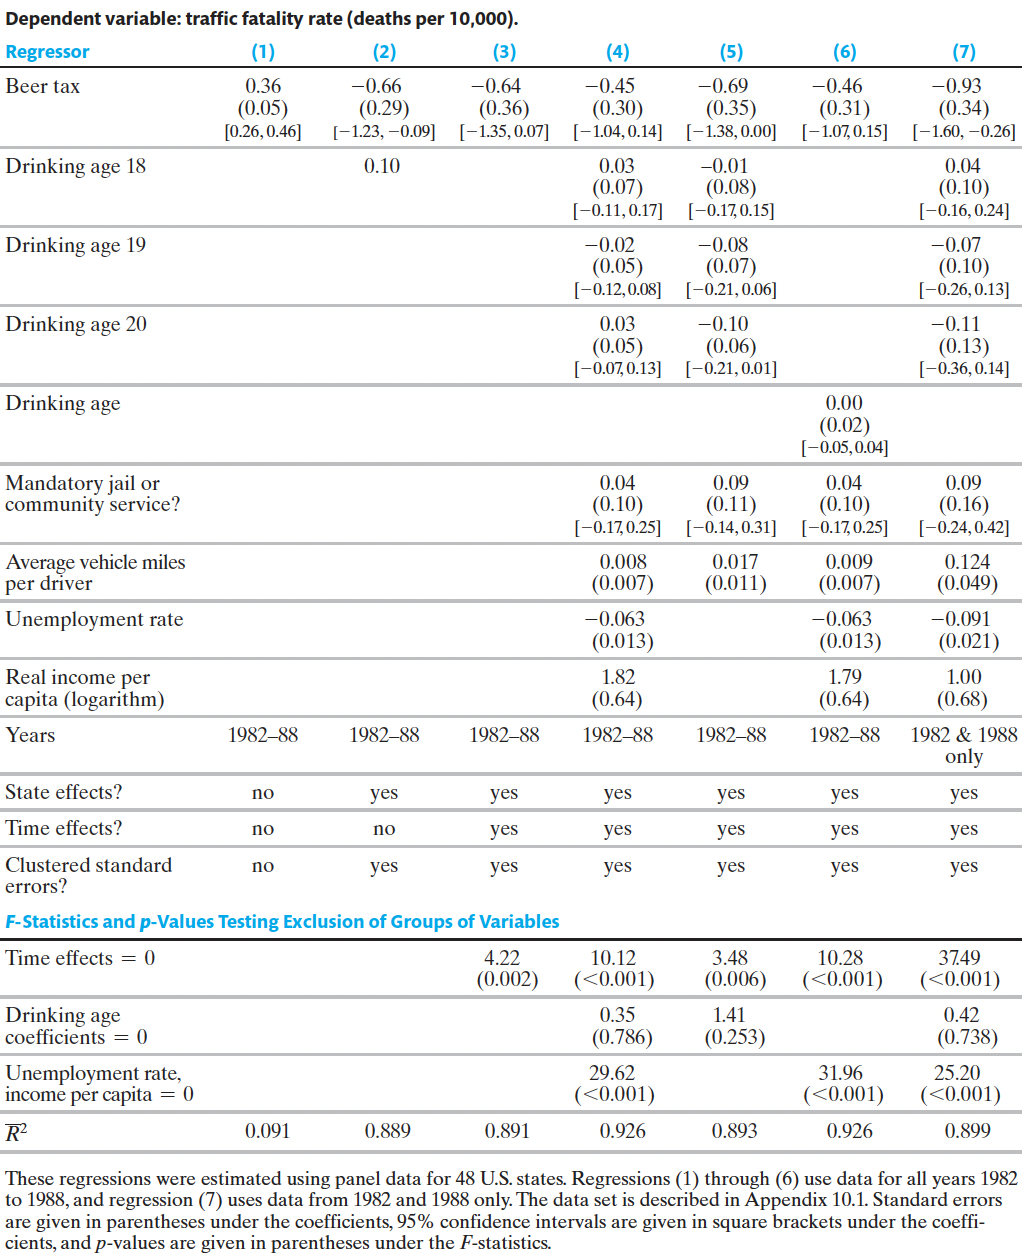
\includegraphics[width=\linewidth]{images/ps6e5.png}
\end{figure}
\end{exercise}

\begin{exercise} % 10.7
Suppose a researcher believes that the occurrence of natural disasters such as earthquakes leads to increased activity in the construction industry. He decides to collect province-level data on employment in the construction industry of an earthquake-prone country, like Japan, and regress this variable on an indicator variable that equals 1 if an earthquake took place in that province in the last five years.
\begin{enumerate}[label=\alph*)]
    \item Should the researcher include province fixed effects in order to control for location-specific characteristics of the labor market?
    \item What can the researcher to control for location effects?
\end{enumerate}
    
\end{exercise}


\begin{exercise} % 10.9
\begin{enumerate}[label=\alph*)]
    \item In the fixed effects regression model, are the fixed entity effects, $\alpha_i$, consistently estimated as $n\rightarrow\infty$ with $T$ fixed?
    \item If $n$ is large (say, $n=2000$) but $T$ is small (say, $T=4$) do you think that the estimated values of ai are approximately normally distributed? Why or why not?
\end{enumerate}
\end{exercise}


\begin{exercise} % 10.11
Let $\beta^{DM}_1$ denote the entity-demeaned estimator seen in class, and let $\beta^{BA}_1$ denote the ``before and after'' estimator without an intercept, so that $\beta^{BA}_1 = \frac{\sum_{i=1}^n (X_{i1}- X_{i2})(Y_{i1}- Y_{i2})}{\sum_{i=1}^n (X_{i1}- X_{i2})^2}$. Show that if $T=2$, $\beta^{DM}_1=\beta^{BA}_1$.
\end{exercise}

\begin{exercise} % 11.1 review of concepts
Suppose a linear probability model yields a predicted value of Y that is equal to 1.3. Explain why this is nonsensical.
\end{exercise}

\begin{exercise} % 11.1-11.5
Seven hundred income-earning individuals from a district were randomly selected and asked whether they are government employees ($Gov_i = 1$) or not ($Gov_i = 0$); data were also collected on their gender ($Male_i = 1$ if male and = 0 if female) and their years of schooling ($Schooling_i$, in years). Note, Schooling refers to the number of years of education received by people ages 25 and older. The following table summarizes several estimated models.
\begin{figure}[htbp]
\caption*{Table 2}
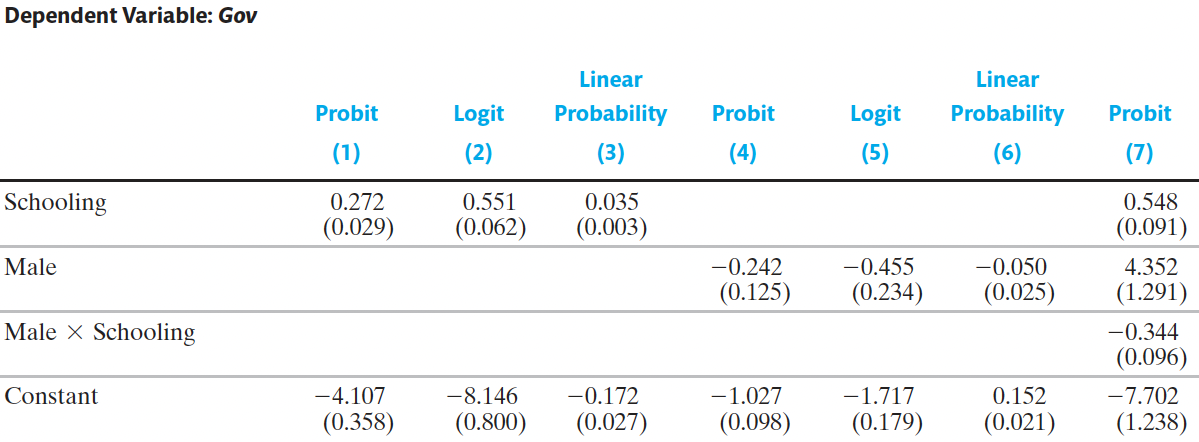
\includegraphics[width=\linewidth]{images/ps6e10.png}
\end{figure}

If need be, you can use the \href{https://engineering.purdue.edu/~reibman/ece302/normal_cdf.pdf}{table of the Standard Normal Cumulative Distribution Function}.
\begin{enumerate}[label=\alph*)]
    \item Using the results in column (1):
        \begin{enumerate}[label=\roman* --]
        \item Does the probability of working for the government depend on Schooling? Explain.
        \item Friedrich F\"rnrohr has 16 years of schooling. What is the probability that he will be employed by the government?
        \item Hans Schneider never went to college (12 years of schooling). What is the probability that Hans will get a government job?
        \item The sample included values of Schooling between 0 and 18 years, and only five people in the sample had more than 15 years of schooling. G\"unter Mayer has completed his PhD and has been a student for 24 years. What is the model's prediction for the probability that G\"unter will be employed by the government? Do you think that this prediction is reliable? Why or why not?
        \end{enumerate}
    \item Answer the previous questions (a.i-a.iv) using column 2.
    \item Sketch the predicted probabilities from the probit and logit in columns (1) and (2) for values of Schooling between 0 and 18. Are the probit and logit models similar?
    \item Answer the previous questions (a.i-a.iv) using column 3.
    \item Sketch the predicted probabilities from the probit and linear probability in columns (1) and (3) as a function of Schooling for values of Schooling between 0 and 18. Do you think that the linear probability is appropriate here? Why or why not?
    \item Using the results in columns (4) through (6):
        \begin{enumerate}[label=\roman* --]
        \item Compute the estimated probability of being employed by the government for men and for women.
        \item Are the models in (4) through (6) different? Why or why not?
        \end{enumerate}
    \item Using the results in column (7):
        \begin{enumerate}[label=\roman* --]
    \item Liam Johansson is a man with 10 years of schooling. What is the probability that government will employ him?
    \item Anneli Karlsson is a woman with 12 years of schooling. What is the probability that government will employ her?
    \item Does the effect of schooling on government employment depend on gender? Explain.
        \end{enumerate}
        \end{enumerate}
\end{exercise}


\end{document}
